\documentclass{beamer}
\usefonttheme[onlymath]{serif}

\usepackage{amsfonts}

% Code Block Setting
\usepackage{listings}
\lstset{language=C,
numberstyle=\footnotesize,
basicstyle=\ttfamily\footnotesize,
numbers=left,
stepnumber=1,
frame=shadowbox,
breaklines=true}

\usetheme{Warsaw}
% \usecolortheme{dove}

% Add frame number and total frame number in footline
\defbeamertemplate*{footline}{shadow theme}{%
    \leavevmode%
    \hbox{\begin{beamercolorbox}[wd=.5\paperwidth,ht=2.5ex,dp=1.125ex,leftskip=.3cm plus1fil,rightskip=.3cm]{author in head/foot}%
            \usebeamerfont{author in head/foot}\hfill\insertshortauthor
        \end{beamercolorbox}%
        \begin{beamercolorbox}[wd=.4\paperwidth,ht=2.5ex,dp=1.125ex,leftskip=.3cm,rightskip=.3cm plus1fil]{title in head/foot}%
            \usebeamerfont{title in head/foot}\insertshorttitle\hfill%
        \end{beamercolorbox}%
        \begin{beamercolorbox}[wd=.1\paperwidth,ht=2.5ex,dp=1.125ex,leftskip=.3cm,rightskip=.3cm plus1fil]{title in head/foot}%
            \hfill\insertframenumber\,/\,\inserttotalframenumber
    \end{beamercolorbox}}%
    \vskip0pt%
}

% Tikz related
\usepackage{tikz}
\usetikzlibrary{fit}
\usetikzlibrary{calc}
\usetikzlibrary{positioning}

% Number the figures
\setbeamertemplate{caption}[numbered]

% Add outline page at begining of each section
\AtBeginSection[]
{
    \begin{frame}<beamer>
        \frametitle{Outline}
        \tableofcontents[currentsection, hideallsubsections]
    \end{frame}
}

%%%%%%%%%%%%%%%%%%%%%%%%%%%%%%%%%%%%%%%%%%%%%

\title{Large scale deep learning parameter server}
\author{
    Ching-Yuan, Tsai
}
\date{
    \tiny{2017,4,26}\\
    \tiny{Presented by Ching-Yuan, Tsai}
}

\begin{document}
\begin{frame}
    \titlepage
\end{frame}

\section{Introduction}

\subsection{SIMD}
\begin{frame}
    \frametitle{SIMD}
	\begin{itemize}
		\item Single instruction multiple data
		\item without threads support
	\end{itemize}
\end{frame}


\subsection{VPU}
\begin{frame}
    \frametitle{VPU}
	\begin{itemize}
		\item Vector processing units 
		\item combine itstructions as vector	
	    \begin{figure}
			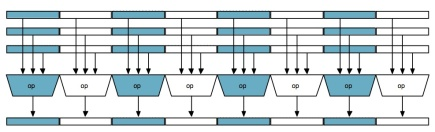
\includegraphics[scale=0.5]{figure/vpu.jpg}
		\end{figure}
	\end{itemize}
\end{frame}


\section{Challenge}

\subsection{Parameters}
\begin{frame}
    \frametitle{Parameters}
	\begin{itemize}
		\item Realistic training models have $10^{9}$ to $10^{12}$ parameters.
		\item Accessing parameters need hight network bandwidth. 
	\end{itemize}
\end{frame}

\subsection{Long idle time}
\begin{frame}
    \frametitle{Long idle time}
	\begin{itemize}
		\item Worker waits unitl server aggregates all parameters.
    	\begin{figure}
			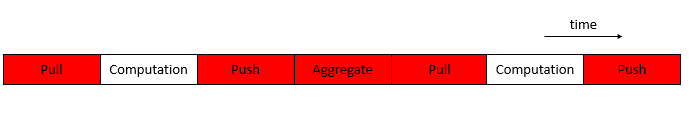
\includegraphics[scale=0.4]{figure/time.png}
		\end{figure}
	\end{itemize}
\end{frame}




\section{(key, value) Vector}

\subsection{Key}
\begin{frame}
    \frametitle{Key}
	\begin{itemize}
		\item Key indicate neural id.
    	\begin{figure}
			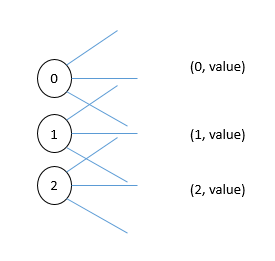
\includegraphics[scale=0.5]{figure/key.png}
		\end{figure}
	\end{itemize}
\end{frame}

\subsection{Value}
\begin{frame}
    \frametitle{Value}
	\begin{itemize}
		\item Value indicate weights with respect to the neural id. 
    	\begin{figure}
			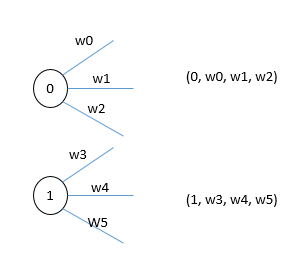
\includegraphics[scale=0.5]{figure/value.png}
		\end{figure}
	\end{itemize}
\end{frame}

\subsection{Vector}
\begin{frame}
    \frametitle{Vector}
	\begin{itemize}
		\item Vector is the combination of key and values.
		\item Vector is the minimum communication unit.
	\end{itemize}
\end{frame}



\section{Range push and pull}

\subsection{Motivation}
\begin{frame}
    \frametitle{Motivation}
	\begin{itemize}
		\item Wokers waste a lot of time to wait network communication and parameter aggregation.
   		\begin{figure}
			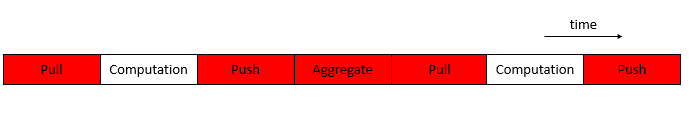
\includegraphics[scale=0.4]{figure/time.png}
		\end{figure}
	\end{itemize}
\end{frame}

\subsection{Idea}
\begin{frame}
    \frametitle{Idea}
	\begin{itemize}
		\item Sending less data to server. 
		\item Sending vectors whose key is within the given range.   
	\end{itemize}
\end{frame}

\subsection{Is it correct ?}
\begin{frame}
    \frametitle{Is it correct ?}
    \begin{figure}
		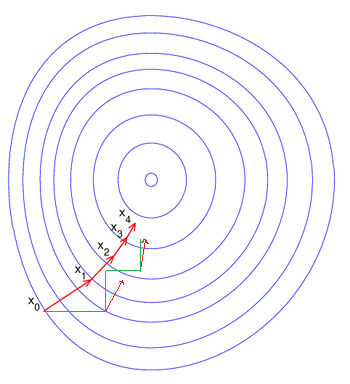
\includegraphics[scale=0.4]{figure/spGD.png}
	\end{figure}
\end{frame}




\section{Reduce idle}

\subsection{Assumption}
\begin{frame}  
    \frametitle{Assumption}
	\begin{itemize}
		\item Computation time is fixed. 
		\item Message communication time decrease as communication range decrease. 
		\item Aggregation time decrease as communication range derease. 
	\end{itemize}
\end{frame}

\subsection{What range size is the best ? }
\begin{frame}
    \frametitle{What range size is the best ?}
	\begin{itemize}
		\item We can decrease size ...
    	\begin{figure}
			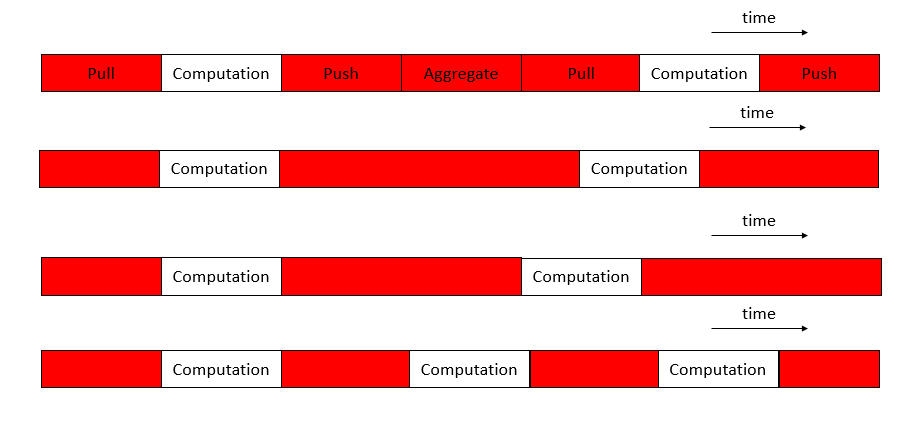
\includegraphics[scale=0.3]{figure/diffsizetime.png}
		\end{figure}
	\end{itemize}
\end{frame}

\subsection{Best size}
\begin{frame}
    \frametitle{Best size}
    \begin{figure}
		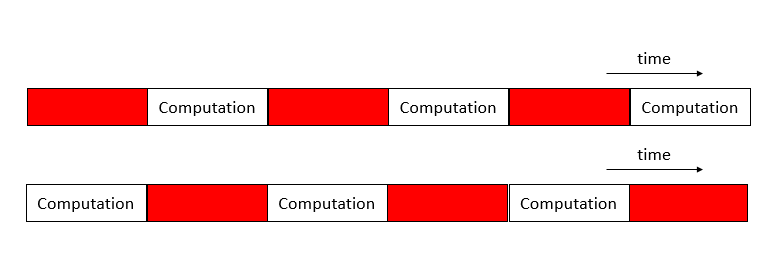
\includegraphics[scale=0.3]{figure/besttime.png}
	\end{figure}
\end{frame}

\subsection{Server view}
\begin{frame}
    \frametitle{Server view}
    \begin{figure}
		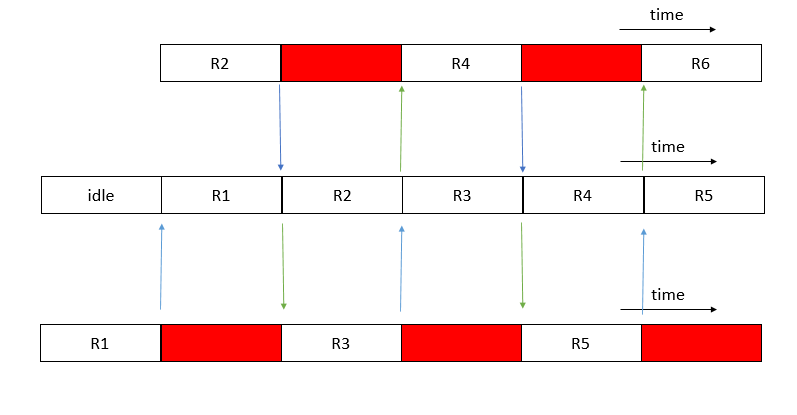
\includegraphics[scale=0.3]{figure/serverview.png}
	\end{figure}
\end{frame}




\section{Mnist model}

%\subsection{Handwritten digits}

\begin{frame}  
    \frametitle{Handwritten digits}
	\begin{itemize}
		\item Subset of a larger set from NIST.
		\item 60000 examples
		\item One color channel
    	\item fixed-size image
	\end{itemize}
\end{frame}

\begin{frame}  
    \frametitle{Handwritten digits}
    \begin{figure}
		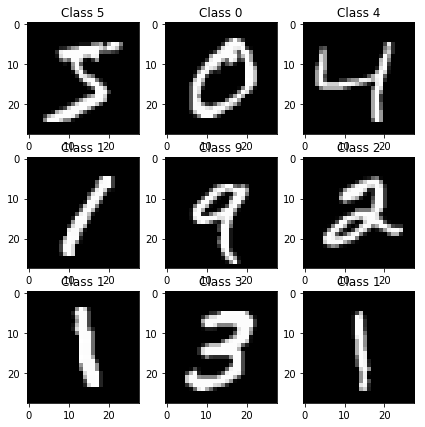
\includegraphics[scale=0.3]{figure/handwritten.png}
	\end{figure}

\end{frame}






\section{Implimentation}

\subsection{Training Model}

\begin{frame}  
    \frametitle{Training Model}
	\begin{itemize}
		\item Use keras
		\item Three dense layers each has 512 neurals
		\item 98 percent accuracy
	\end{itemize}
\end{frame}

\begin{frame}
	\frametitle{Training Model}
	\begin{figure}
		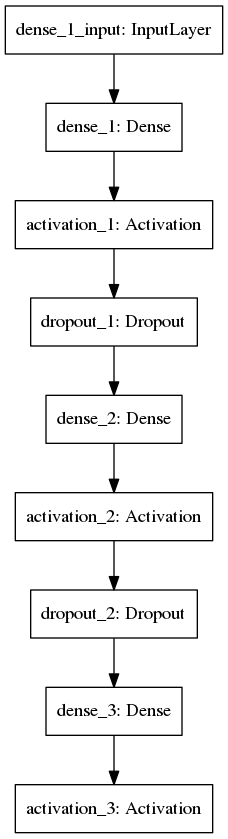
\includegraphics[scale=0.2]{figure/model_structure.png}
	\end{figure}
\end{frame}
\subsection{Server Synchronization}
\begin{frame}  
    \frametitle{Server Synchronization}
	\begin{itemize}
  		\item Synchronize client iterations	
		\item Python client, C server
		\item Two states machine		
		\begin{itemize}
  			\item Push state
			\item Pull state	
		\end{itemize}
	\end{itemize}
\end{frame}





\section{Future work}

\subsection{Future work}
\begin{frame}
    \frametitle{Future work}
	\begin{itemize}
		\item How to fit computation time and message communication time. 
		\item If Computation time is not fixed. 
		\item Implement parameter server. 
	\end{itemize}
\end{frame}




\section{Stale Synchronous Parallel}

\subsection{Sliding Window Method}
\begin{frame}  
    \frametitle{Sliding Window}
	\begin{itemize}
		\item Sliding Window is an integer range indicating the valid interations.
		\item Clients can not push parameters with the invalid interations. 
		\item Server checks the low bound of the sliding window when the clients push parameters. 
		\item Shift the sliding window. 
	\end{itemize}
\end{frame}


\begin{frame}
    \frametitle{Sliding Window}
	\begin{itemize}
		\item Time complexity
			\begin{itemize}
				\item Clients push parameters: $O(1)$
				\item Server check low bound: $O(1)$
			\end{itemize}
		\item Space complexity: $O(l)$ which l is the length of the sliding window.
			\begin{itemize}
				\item Independent on the \# of clients thus has good scalibility. 
			\end{itemize}
	\end{itemize}
\end{frame}

\subsection{Parallel SGD}
\begin{frame}
    \frametitle{BSP}
    \begin{itemize}
		\item Bulk Synchrnous Parallel
		\item Clients can not continue to the next iteration until the server receives all gradients.
		\item It guarantees converage. 
	\end{itemize}
\end{frame}

\begin{frame}
    \frametitle{ASP}
    \begin{itemize}
		\item Asynchronous Parallel
		\item Clients continue to the next iteration without waiting for each other. 
		\item It may not converage. 
		\item It can be up to 10X slower when the heterogeneity increase.
	\end{itemize}
\end{frame}

\begin{frame}
    \frametitle{SSP}
    \begin{itemize}
		\item Stale Synchrnous Parallel
		\item The faster client can not go ahead the slowest one more than a predefined staleness. 
		\item SGD usually uses this method. 
		\item It can be slower when the heterogeneity increase.
	\end{itemize}
\end{frame}

\begin{frame}
    \frametitle{Constant learning rate, Dynamic learning rate}
    \begin{itemize}
		\item CONSGD
		\begin{itemize}
			\item A constant global learning rate and multiplies it to each local update.
		\end{itemize}
		\item DYNSGC
		\begin{itemize}
			\item To further improve performance over CONSGD.
			\item Server dynamic update global learning rate basing on maximun staleness.
		\end{itemize}
	\end{itemize}
\end{frame}

%\subsection{Server view}
%\begin{frame}
%    \frametitle{Server view}
%    \begin{figure}
%		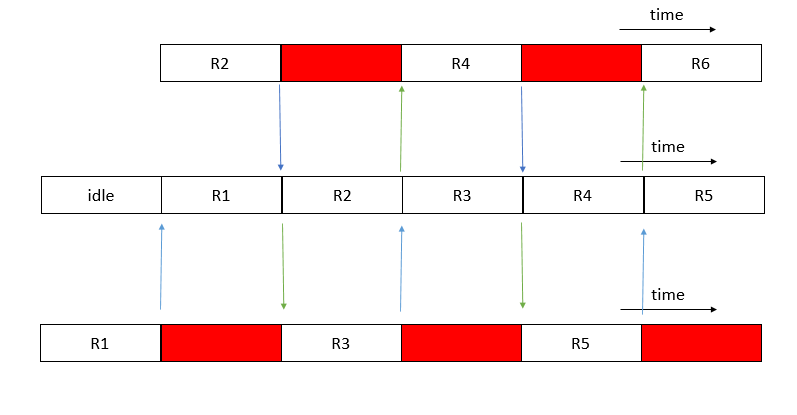
\includegraphics[scale=0.3]{figure/serverview.png}
%	\end{figure}
%\end{frame}




\section{Global learning rate with SSP SGD}
\subsection{Angel Parameter Server}
\begin{frame}
    \frametitle{Constant learning rate, Dynamic learning rate}
    \begin{itemize}
		\item CONSGD
		\begin{itemize}
			\item A constant global learning rate and multiplies it to each local update.
		\end{itemize}
		\item DYNSGC
		\begin{itemize}
			\item To further improve performance over CONSGD.
			\item Server dynamic update global learning rate basing on maximun staleness.
		\end{itemize}
	\end{itemize}
\end{frame}

\begin{frame}
	\frametitle{Things they do not consider}
	\begin{itemize}
		\item The workers with smaller interations have larger local learning rate.
			\item $w_{t+1} = w_{t}+\frac{\eta}{\sqrt{\sum_{i<=t+1}(g_{i})^2}}g_{t+1}$
	\end{itemize}
\end{frame}

\subsection{Spliting gradients}
\begin{frame}
	\frametitle{Spliting gradients}
	\begin{itemize}
		\item Spliting gradient into 'direction' and 'distance'.
			\begin{itemize}
				\item Distance: $|gradient|$.
				\item Dircetion: $\frac{gradient}{|gradient|}$
				\item Gradient = Distance * Direction
			\end{itemize}
		\item Scheduling distance of each gradient.
		\begin{itemize}
			\item Do not change the distance of the sum of all latest gradients of each worker.
		\end{itemize}
	\end{itemize}
\end{frame}

\begin{frame}
	\frametitle{Computing distances}
	\begin{itemize}
		\item Server computes the the following $t$ when push commands occur.
			\begin{itemize}
				\item $t|\sum_{i=0}^{M}\alpha_{c}\frac{g_{c}^{i}}{|g_{c}^{i}|}|=|\sum_{i=0}^{M}g_{c}^{i}|$
			\end{itemize}
		\item $t*\alpha_{c}$ is the new distance of $g_{c}^{i}$
	\end{itemize}
\end{frame}
%\subsection{Server view}
%\begin{frame}
%    \frametitle{Server view}
%    \begin{figure}
%		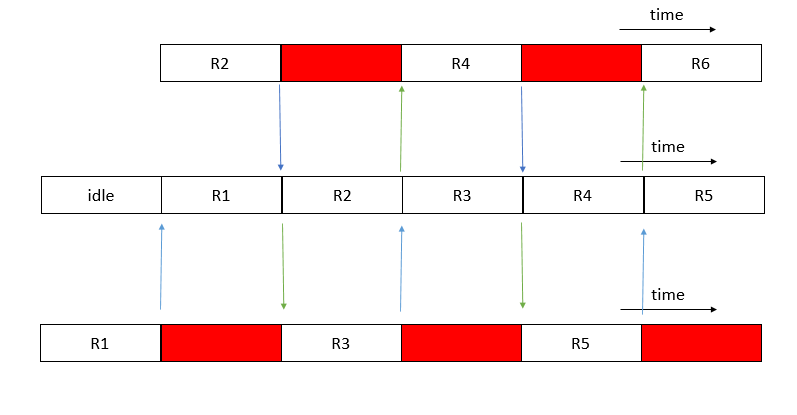
\includegraphics[scale=0.3]{figure/serverview.png}
%	\end{figure}
%\end{frame}




\end{document}
